 \documentclass{report}
 
\usepackage[utf8]{inputenc} 
\usepackage[T1]{fontenc}      
\usepackage[top=3.5cm, bottom=3cm, left=3.0cm, right=4.0cm]{geometry}
\usepackage{graphicx}
\usepackage{amsmath}
\graphicspath{{figures/}{../figures}}

\begin{document}

\section*{Exercice 1}

On s'intéresse à l'écoulement stationnaire, incompressible d'un fluide de masse volumique $\rho$ et de viscosité $\eta$ autour d'une sphère de rayon $R$. La vitesse de l'écoulement loin de la sphère est $v_\infty\vec{e_z}$. On adoptera les coordonnées sphériques d'axe $Oz$, $O$ étant le centre le centre de la sphère. 

\begin{itemize}
	\item[•] On suppose que l'écoulement permet de négliger le terme convectif de l'équation de Navier-Stokes devant le terme diffusif. Comment s'écrit alors cette équation ? 
	\item[•] On suppose que la vitesse est telle que : $\vec{rot}(\vec{rot}(\vec{v}))=\frac{3v_\infty R}{r^3}\left(\cos\theta\vec{e_r}+\frac{1}{2}\sin\theta\vec{e_\theta} \right) $. Quelle est la résultante des forces de pression sur la sphère ? 
	\item[•] Quelle est la résultante des actions de cisaillement sur la sphère ? On donne $\left(\frac{\partial v_\theta}{\partial r}\right)_{r=R}=\frac{3v_\infty}{2R}\sin\theta  $.
	\item[•] Trouver la force de trainée s'exerçant sur la sphère. 
\end{itemize}

On donne : 
\begin{equation}
	\Delta f = \frac{1}{r^2}\frac{\partial}{\partial r} \left(r^2\frac{\partial f}{\partial r} \right) + \frac{1}{r^2\sin\theta}\frac{\partial}{\partial \theta} \left(\sin\theta\frac{\partial f}{\partial \theta} \right) + \frac{1}{r^2\sin^2\theta}\frac{\partial^2 f}{\partial \varphi^2} 
\end{equation}

\begin{equation}
	\vec{grad} f = \frac{\partial f}{\partial r} \vec{e_r} + \frac{1}{r}\frac{\partial f}{\partial \theta}\vec{e_\theta} + \frac{1}{r\sin\theta}\frac{\partial f}{\partial \varphi}\vec{e_\varphi}
\end{equation}

\newpage

\section*{Exercice 2}

On considère un fluide d'épaisseur $h$ s'écoulant lentement sur un plan infini incliné d'un angle $\alpha$ par rapport à la verticale. Le fluide a une forte viscosité $\eta$ et une masse volumique $\rho$, et il est soumis à la gravité. On est en régime permanent.

\begin{center}
	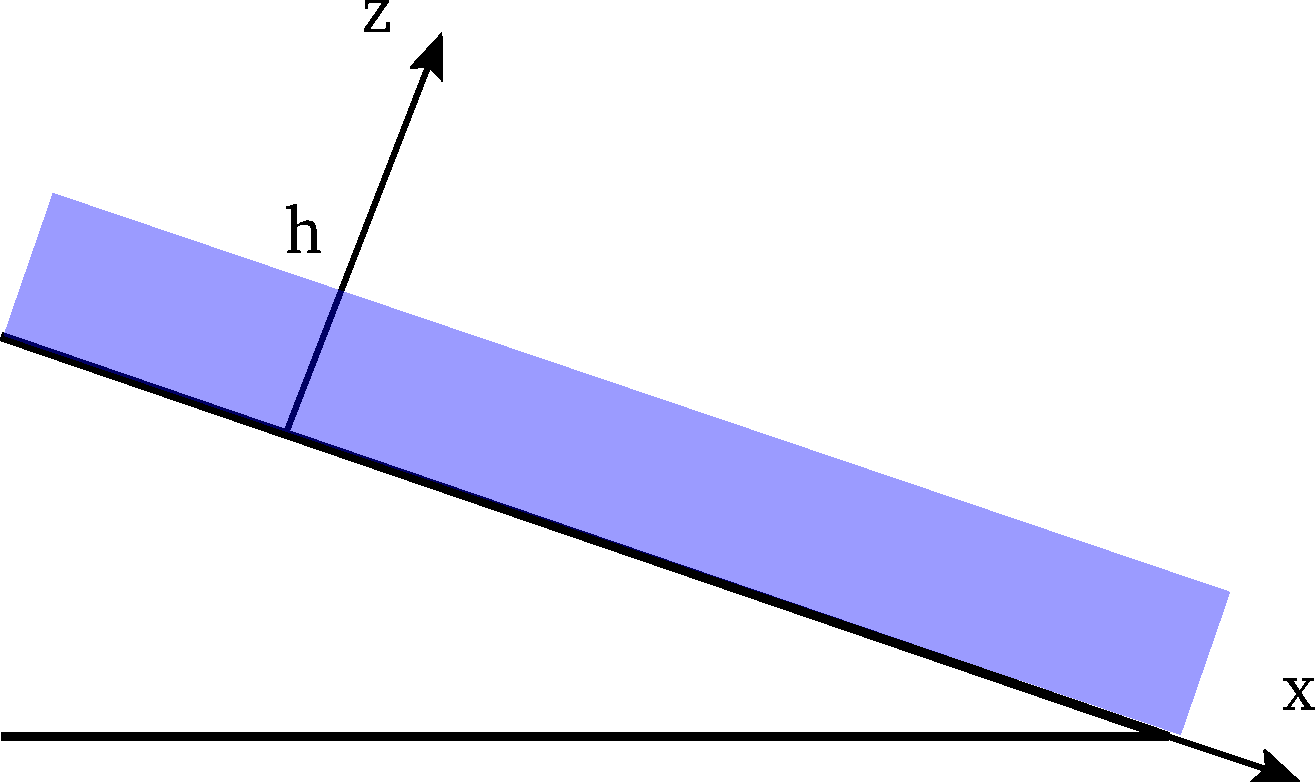
\includegraphics[scale=0.3]{ecoulement.pdf}
\end{center}

\begin{itemize}
	\item[1 -] Quel est le profil de vitesse dans le fluide ? 
	\item[2 -] En déduire le débit. 
	\item[3 -] On observe avec des images satellite que la vitesse d'écoulement d'un glacier à sa surface est d'environ 100m/an. En déduire la viscosité d'un glacier de 100m d'épaisseur, d'un kilomètre de large. Quelle quantité de glace est charriée en une année ?
	\item[5 -] On place désormais une plaque au dessus du liquide, au niveau de $z=h$. Que deviennent les conditions aux limites ? Trouver le nouveau profil de vitesse. Comment s'appelle se type d'écoulement ?

\end{itemize}

\newpage

\section*{Exercice 3}

On étudie un écoulement permanent d'un fluide incompressible de masse volumique $\mu$, dans un tuyau cylindrique horizontal d'axe $Oz$, de rayon $R$, et de longueur $L$ (schéma de gauche). Le champ de pression appliqué le long du tube est noté $P(r,z)$. Par invariance, le champ de vitesse est supposé ne dépendre que de $r$ et $z$, et est dirigé selon $\vec{e_z}$. Il est noté $\vec{u}=u(r,z)\vec{e_z}$. On définit la vitesse de cisaillement par la quantité $\dot{\gamma}=-\frac{du}{dr}$. 

\begin{center}
	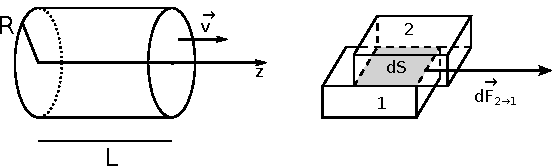
\includegraphics[scale=0.8]{meca_flu2.pdf}
\end{center}

On définit la force surfacique de viscosité $\vec{\tau}$, ou contrainte de cisaillement, entre deux couches adjacentes de fluide, la quantité : $\vec{\tau}=\frac{d\vec{F}}{dS}$.
où $d\vec{F}$ est la force qui s'exerce mutuellement entre les couches adjacentes, et $dS$ la surface élémentaire de contact entre ces deux surfaces (schéma de droite).

\begin{itemize}
	\item[1 - ] Quelle est la relation entre la force de viscosité $\vec{\tau}$ et le champ de vitesse $u$ dans le cas d'un fluide classique (vu en cours), dit newtonien ? On pourra dans cette question se placer en coordonnées cartésiennes.
	
\end{itemize}

\subsubsection*{Fluide de Bingham}

Un fluide est dit de Bingham si les contraintes de cisaillements entre les couches obéissent à une loi de seuil : 
\begin{align*}
	\left\lbrace
\begin{array}{ccc}
\tau>\tau_s & : & \tau = \tau_s+\eta\dot{\gamma} \\
\tau<\tau_s & : & \dot{\gamma}=0\\
\end{array}\right.
\end{align*}
On supposera que le fluide que l'on étudie obéit à une telle loi. 

\begin{itemize}
	\item[2 - ] Quel est la différence entre un fluide classique et un fluide de Bingham ?

	\item[3 - ] Montrer que $\vec{u}$ ne dépend que de $r$. En négligeant les actions de la pesanteur, déterminer la relation suivante : 
	\begin{align*}
		\frac{\partial P}{\partial z} + \frac{1}{r}\frac{\partial (r\tau)}{\partial r}=0
	\end{align*}
	\item[4 - ] Établir la relation :
	\begin{align*}
		\tau(r) = \tau_s\frac{r}{R_s}
	\end{align*}
	où $R_s$ est le rayon de seuil, défini par $R_s=2\tau_s L/\Delta P$, en notant $\Delta P = P(0)-P(L)$ la chute de pression entre l'entrée et la sortie du tuyau. Quel est le signe de $\Delta P$ ?

	\item[5 - ] Pour quelle pression minimale $\Delta P_{min}$ commence t-on à voir un écoulement à travers le tube ?
	
	\item[6 - ] On suppose que $\Delta P>\Delta P_{min}$. Déterminer le champs de vitesse dans le tube. Tracer son allure et expliquer pourquoi l'écoulement présente une zone dite \textit{bouchon}.
	
	
\end{itemize}

\newpage

\section*{Exercice 4}

\subsubsection*{Tuyau parabolique}

Un fluide est en écoulement permanent dans une portion de tube à section parabolique, avec $Oz$ en axe de symétrie. Les lignes de courant s'écoulant dans le tube ont pour équation :
\begin{align*}
		\left\lbrace
\begin{array}{ccc}
z<0 & : & r=\lambda a \\
z>0 & : & r=\lambda \left(a+\frac{z^2}{b} \right) \\
\end{array}\right.
\end{align*}
où $\lambda$ est un nombre sans dimension, $a$ et $b$ des constantes. 

\begin{center}
	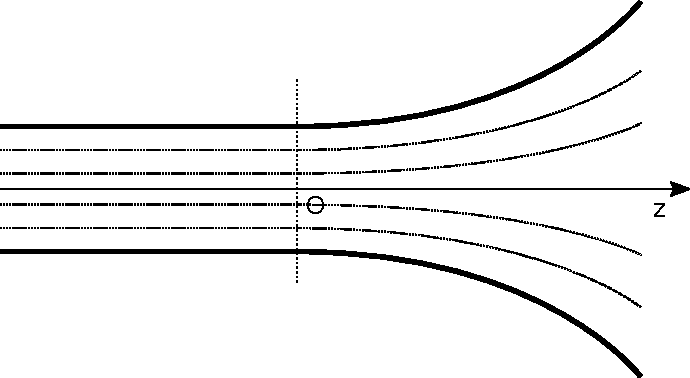
\includegraphics[scale=0.5]{meca_flu1.pdf}
\end{center}

Le fluide est incompressible et la composante axiale de $v_z$ de la vitesse est supposée uniforme sur une section perpendiculaire, cad $v_z$ ne dépend pas de $r$. On note $v_0$ la vitesse en $O$.

\begin{itemize}
	\item[1 - ] Déterminez la vitesse $\vec{v}$ en tout point.
	\item[2 - ] Comment évolue un élément de fluide qui traverse le tuyau ? 
	\item[3 - ] L'écoulement est-il potentiel ?
\end{itemize}

\subsubsection*{Écoulement entre deux lames}

On considère deux plaques infinies de verres séparées d'une épaisseur $e$ où circule un fluide incompressible. Du fluide est injecté à un débit $D_e$ par le tuyau $A$, et il peut ressortir à travers le tuyau $B$ identique. 

On suppose que l'écoulement dérive du potentiel :
\begin{align*}
	\phi(M) = av_0\ln\frac{r_A}{r_B}
\end{align*}
où $r_A$ (resp. $r_B$) est la distance d'un point $M$ du champ à la source $A$ (resp. $B$).

\begin{center}
	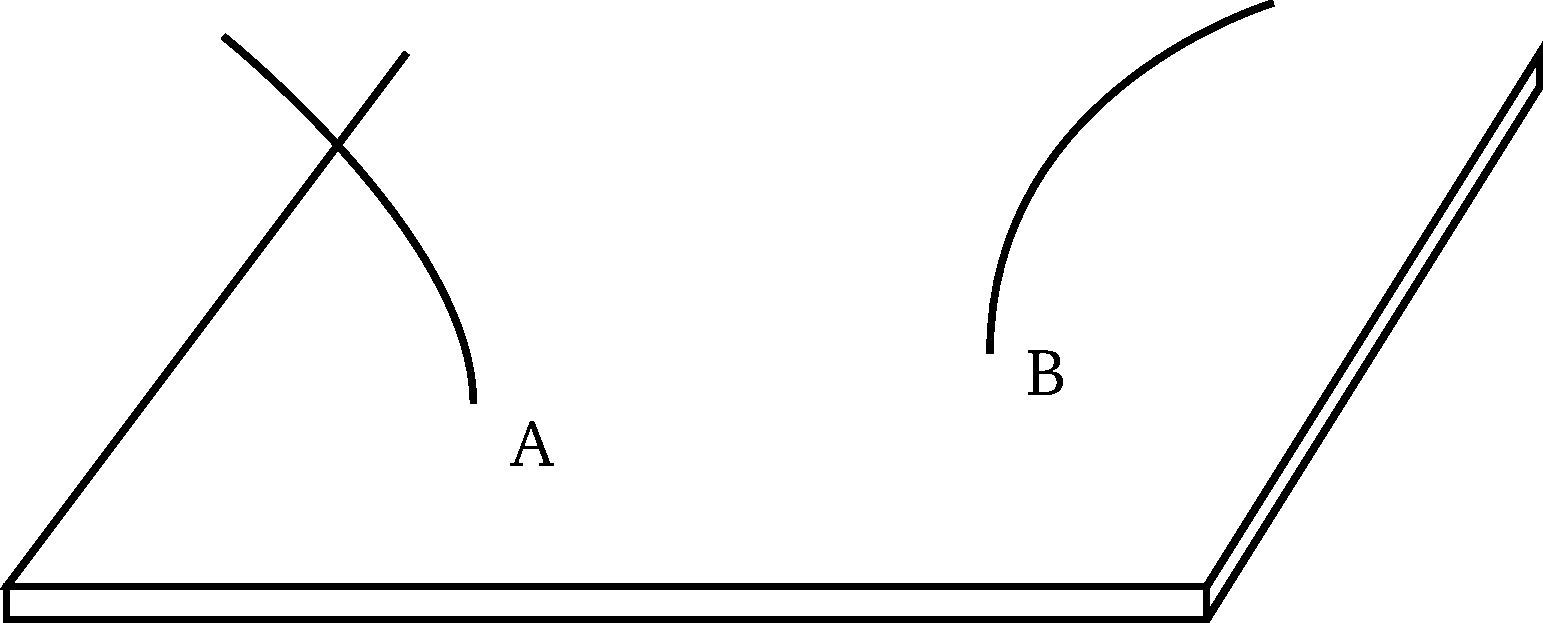
\includegraphics[scale=0.25]{plaque.pdf}
\end{center}

\begin{itemize}
	\item[1 - ] Déterminer le champ des vitesses. Comment relier $a$ et $v_0$ au débit des sources ? 
	\item[2 - ] Est-ce un écoulement compressible ?
\end{itemize}

\newpage

\section*{Exercice 5}

On considère un fluide incompressible, de viscosité $\eta$ contenu entre deux cylindres orientés verticalement, de même axe $O_z$, et de rayons respectifs $R_1$ et $R_2$ (avec $R_1<R_2$). La hauteur des cylindres $L$ est très grande devant les rayons : $L\gg R_1, R_2$. Les deux cylindres peuvent tourner autour de l'axe $Oz$. 

\begin{center}
	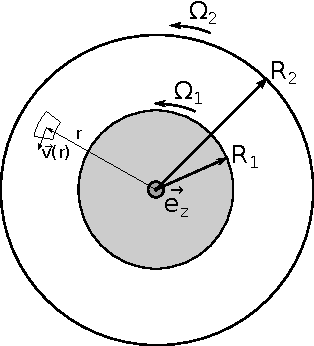
\includegraphics[scale=0.8]{meca_flu3.pdf}
\end{center}

Tout élément de ce fluide subit une force surfacique visqueuse (ou contrainte visqueuse) que l'on notera $\vec{\sigma}$. L'expression en coordonnées cylindrique de sa composante selon $\vec{e_\theta}$ s'écrit : 
\begin{align*}
	\sigma_\theta(r,\theta,z)=\eta\left(\frac{1}{r}\frac{\partial v_r}{\partial \theta}+ \frac{\partial v_\theta}{\partial r} - \frac{v_\theta}{r} \right)
\end{align*}
Il est possible de démontrer que, dans le cadre de ce problème, les autres composantes de $\vec{\sigma}$ sont nulles. Nous l'admettrons pour la suite du problème. 

L'écoulement est supposé permanent, lent et laminaire : on suppose alors que $v_z=0$.

\begin{itemize}
	\item[1 - ] A partir des invariances du problèmes, montrer que $v$ ne dépend que de $r$.

	\item[2 - ] En s'appuyant sur un bilan de matière, retrouver l'expression de l'équation de conservation. En déduire que le champ de vitesse s'écrit $\vec{v}=v_\theta (r)\vec{e_\theta}$. L'écoulement est-il rotationnel ?
	
	\item[3 - ] En faisant un bilan des moments selon $\vec{e_z}$, montrer que la vitesse vérifie la relation suivante : 
	\begin{align*}
		\frac{\partial}{\partial r}\left(r^3 \frac{\partial}{\partial r}\frac{v_\theta}{r} \right) =0
	\end{align*}
	
	\item[4 - ] Le cylindre de rayon $R_1$ (resp. $R_2$) tourne à la vitesse angulaire $\Omega_1$ (resp. $\Omega_2$). En déduire l'expression du champs de vitesse. 
	
	\item[5 - ] On suppose que le cylindre intérieur (de rayon $R_1$) est maintenu fixe (cad $\Omega_1=0$) à l'aide d'un ressort de torsion qui exerce un moment $\vec{M}=k\theta\vec{e_z}$. Le cylindre intérieur tourne toujours à la vitesse $\Omega_2$. De quel angle $\theta$ tourne le ressort ? A quel quantité physique a t-on alors accès ?
	
	\item[6 - ] En étant toujours dans la situation $\Omega_2=0$, calculer la puissance mécanique dissipée dans le fluide.
	
\textit{NB} 
\begin{align*}
	\vec{rot}(\vec{v})=\left( \frac{1}{r}\frac{\partial v_z}{\partial\theta}-\frac{v_\theta}{\partial z}\right)\vec{e_r} + \left( \frac{\partial v_r}{\partial z}-\frac{\partial v_z}{\partial r}\right)\vec{e_\theta} + \frac{1}{r}\left( \frac{\partial (rv_\theta)}{\partial r}-\frac{\partial v_r}{\partial \theta}\right)\vec{e_z} 
\end{align*}	
	
	
\end{itemize}

\end{document}
